\newpage
\chapter{Scientific Computing}
\label{chapter01}

Even at the dawn of modern computing, the essential calculations were of a scientific and military nature. This fact has mostly stayed the same in recent decades. Even today, the most computing resources are directed at science. This gives reason to find ways to perform scientific computations even on computing devices not intended for scientific purposes.

\section{Sequential Programming}

In sequential programming\index{sequential programming}, each computational instruction follows all previous ones. At the dawn of computing, calculations were done this way. Even today, a significant proportion of algorithms are executed only sequentially because each instruction's input data depends on the preceding instructions' output data. Sequential algorithms are not decomposable and, therefore, inapplicable to parallel computations (Fig. \ref{fig:pic0001}).

\begin{figure}[h]
\centering
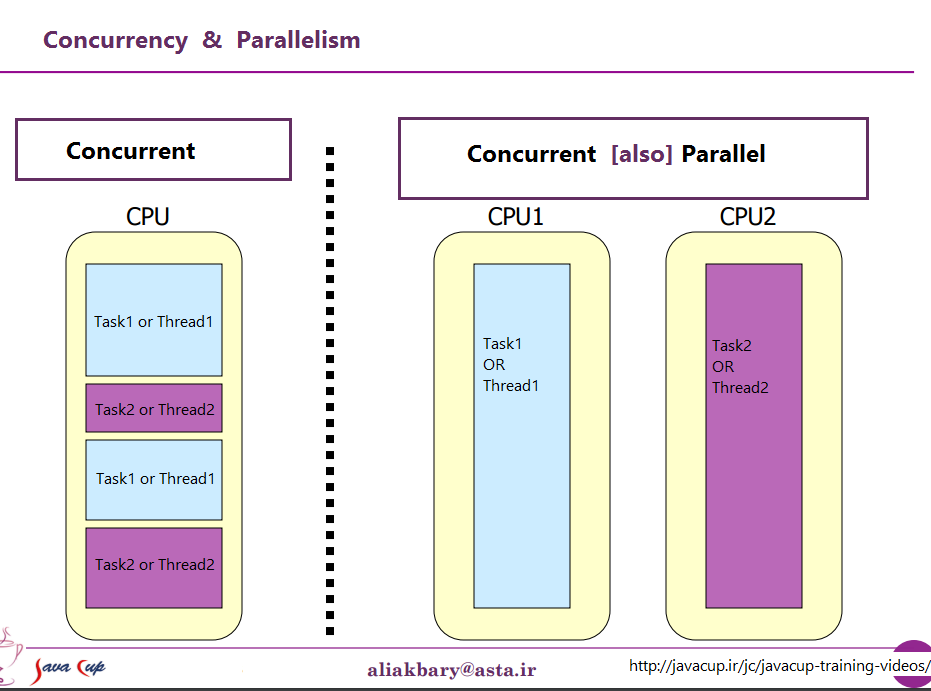
\includegraphics[width=1.0\linewidth]{pic0001}
\caption{Comparison between Sequential Computation and Parallel Computation}
\label{fig:pic0001}
\end{figure}

\section{Parallel Programming}

In parallel programming, there are mainly two varieties - concurrent computations\index{concurrent computations} and parallel computations\index{parallel computations}. Concurrent computations are in an environment where a group of tasks can be computed simultaneously regardless of the calculation order. Parallel computations refer to the simultaneous computation of separate tasks on separate processors. In this context, all parallel computations are concurrent computations, but not vice versa (Fig. \ref{fig:pic0002}).

\begin{figure}[h]
\centering
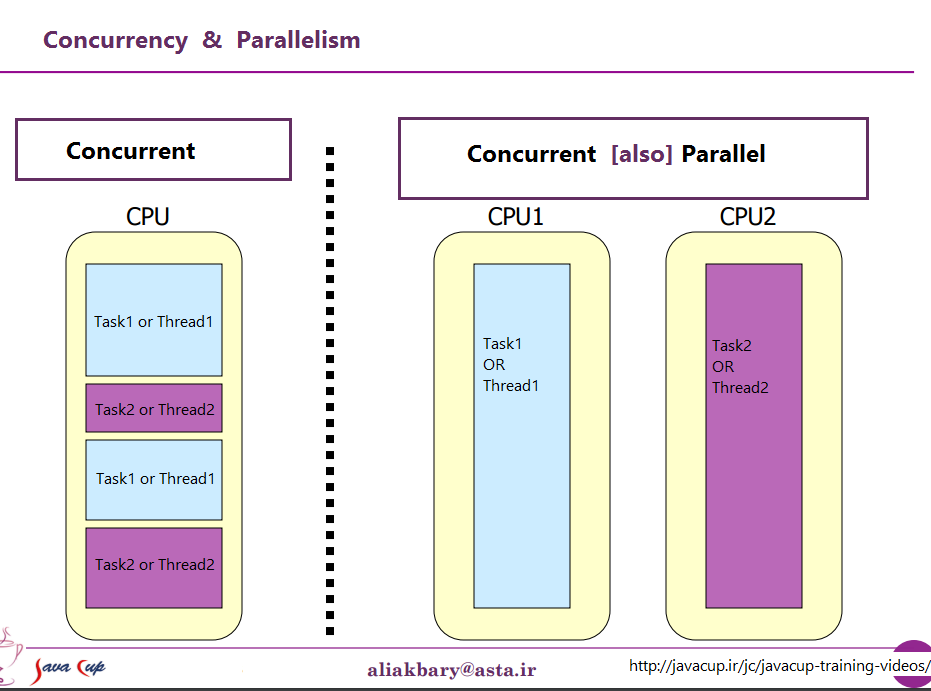
\includegraphics[width=1.0\linewidth]{pic0002}
\caption{Comparison between sequential computations and parallel computations}
\label{fig:pic0002}
\end{figure}

\section{Supercomputing and Grid Computing}

When parallel algorithms are executed on computing machines with multiple processors and/or multiple processor cores, this type of computing is referred to as supercomputing. The essential thing about this kind of computation is that it uses a high-speed internal bus (sometimes optical) and shared RAM. Unlike supercomputers\index{supercomputing}, grid computing\index{grid computing} takes place on multiple machines connected in a standard network but operating autonomously without sharing common memory. In grid systems, individual computing machines can be geographically distant from each other. It is important to note that even with supercomputers\index{supercomputer computing}, the system's owner has complete control over it. This may be slightly different for grid systems if computers under foreign control are connected to the grid.

\section{Computing in a distributed environment}

The transition from grid systems to distributed computing systems\index{distributed computing} is that the computing machines in the distributed environment are autonomous. These machines do not share common resources such as CPU or RAM. It is very characteristic in the distributed environment that the control over the computing machines is not on the side of the organizer of the calculations. This leads to two main problems - unreliable (often too slow) communication and lack of guarantee for the correctness of calculations (manipulations by the owner of the computing resources). Also, in grid systems, there is often a homogeneity of computing resources in terms of hardware configurations and operating systems. In contrast, computing machines are fundamentally heterogeneous in a distributed environment, which can lead to significant differences in hardware and operating systems.

\section{Donated computing power}

For solving more significant scientific problems, computing power and/or financial resources are often insufficient. In such situations, some scientific institutions resort to so-called donated computing resources\index{donated computing resources} in a distributed environment\index{computing in a distributed environment}. One of the most comprehensive lists of projects of this kind can be found at the Distributed Computing Info \cite{dcinfo} website. It is important to note that only some computing problems are suitable for solving in a distributed environment\index{distributed computing} with donated computing power. First, the problem must be decomposable so separate parts can be calculated simultaneously. The second important thing is that it is optional at what point and in what order the computed results will be obtained. And the third essential thing is to have a mechanism for verifying the credibility of the calculations since the calculations are performed on machines with different hardware configurations and operating systems, and manipulations by the people owning these machines are also possible. The most famous project for donated computing power is SETI@home \cite{shuch}, whose goal is to search for signals from space created by intelligent life forms.

When computing occurs on mobile devices, the distributed environment becomes a mobile distributed computing environment\index{mobile distributed computing environment}. The rest of this tutorial will present how to build a system to perform distributed computing on mobile devices.
